\documentclass{beamer}
\usepackage[english,activeacute]{babel}
\usepackage[utf8]{inputenc}
\usepackage{listings}
\usepackage{color}
\usepackage{tikz}
\usepackage{graphicx}
\usepackage{hyperref}
\usepackage{breqn}
\usepackage{amsmath}
\usepackage{amssymb}
\usepackage{caption}
\usepackage{float}

\definecolor{red}{RGB}{255,0,0}
\definecolor{green}{RGB}{0,255,0}
\definecolor{dgreen}{RGB}{118,151,53}
\definecolor{blue}{RGB}{0,0,255}
\definecolor{oran}{RGB}{255,93,0}

\newcommand{\blue}{\textcolor{blue}}
\newcommand{\red}{\textcolor{red}}
\newcommand{\green}{\textcolor{green}}
\newcommand{\dgreen}{\textcolor{dgreen}}
\newcommand{\oran}{\textcolor{oran}}
\newcommand{\gray}{\textcolor{gray}}
\definecolor{gray97}{gray}{.97}
\definecolor{gray75}{gray}{.75}
\definecolor{gray45}{gray}{.45}

%\renewcommand\mathfamilydefault{\rmdefault}
\setbeamertemplate{blocks}[rounded][shadow=true]

\usetheme[pageofpages=of,
          alternativetitlepage=true,
          titlepagelogo=img/aei.png,
          watermark=,
          watermarkheight=50px,
          watermarkheightmult=1,
          ]{Torino}

\lstset{
     frame=single,
     framerule=0pt,
     aboveskip=0.5cm,
     framextopmargin=3pt,
     framexbottommargin=3pt,
     framexleftmargin=0.4cm,
     framesep=0pt,
     rulesep=.4pt,
     backgroundcolor=\color{gray97},
     rulesepcolor=\color{black},
     language=C,
     showstringspaces = false,
     basicstyle=\scriptsize\ttfamily,
     keywordstyle=\bfseries\color{green!70!black},
     commentstyle=\itshape\color{purple},
     %identifierstyle=\color{red},
     stringstyle=\color{orange},
     %commentstyle=\color{gray45},
     %keywordstyle=\bfseries,
     numbers=left,
     numbersep=13pt,
     numberstyle=\scriptsize,
     numberfirstline = false,
     breaklines=true,
     emph = {[1]\_\_device\_\_, \_\_global\_\_, \_\_syncthreads,
             pragma, omp, parallel, private, threadIdx, blockDim, blockIdx,
             cudaThreadSynchronize, while, total, main,dim3},
     emphstyle={[1]\color{blue!70!black}},
   }

% minimizar fragmentado de listados
\lstnewenvironment{listing}[1][]{\lstset{#1}\pagebreak[0]}{\pagebreak[0]}

\lstdefinestyle{consola}{basicstyle=\scriptsize\bf\ttfamily,
                         backgroundcolor=\color{gray75},
                        }



\usecolortheme{nouvelle}
\author[C. Maureira]
       {\Large Cristián Maureira
       \\\normalsize Dr. Pau Amaro-Seoane
       }
\title[GPU {\nbody} integrator]
      {A modular, GPU-based, direct-summation\newline $N-$body integrator}
\institute[AEI]{Albert Einstein Institute}

\let\sun=\odot
\newcommand{\SgrA}{Sgr~A$^\ast$}
\newcommand{\GR}{{\sc Gravidy }}
\newcommand {\MBH}{\ensuremath{M_{\mathrm{BH}}}}
\newcommand {\mbh}{\ensuremath{M_{\mathrm{BH}}}}
\newcommand {\Msun}{\ensuremath{M_{\odot}}}
\newcommand {\msun}{\ensuremath{M_{\odot}}}
\newcommand {\msol}{\ensuremath{M_{\odot}}}
\newcommand {\Mstar}{\ensuremath{M_{\ast}}}
\newcommand {\Rsun}{\ensuremath{R_{\odot}}}
\newcommand {\Mpthree}{\ensuremath{M_{\odot}\,\mathrm{pc}^{-3}}}
\newcommand {\RS}{\ensuremath{R_{\mathrm{S}}}}
\newcommand {\kms}{\ensuremath{\mathrm{km\,s}^{-1}}}
\newcommand {\peryr}{\ensuremath{\mathrm{yr}^{-1}}}
\newcommand{\gr}{gravitational radiation}
\newcommand{\gw}{gravitational waves}
\newcommand{\rem}[1]{} % pour mettre des commentaires en ligne...
\newcommand{\nbody}{$N$-body}
\newcommand{\bs}{\boldsymbol}
\newcommand{\todo}{\textcolor{red}{TO DO:}}

\begin{document}

%\bibliographystyle{unsrt}
%\pagestyle{empty}

% First slide
\begin{frame}[t,plain]
    \titlepage
\end{frame}

% Outline
\begin{frame}
    \frametitle{Contents}
    \tableofcontents
\end{frame}


\section{Introduction}
\section{Introduction}

\begin{frame}
    \frametitle{Introduction}
    \framesubtitle{Motivation (1/2)}

    \begin{columns}
        \begin{column}{0.6\textwidth}
            \begin{itemize}
                \item Dynamical evolution of a dense stellar systems.
                      ({\nbody} Problem)
                \item Newtonian systems compounded by \blue{more than two stars},
                      needs numerical approaches.
            \end{itemize}
        \end{column}
        \begin{column}{0.4\textwidth}
            \begin{figure}
                \centering
                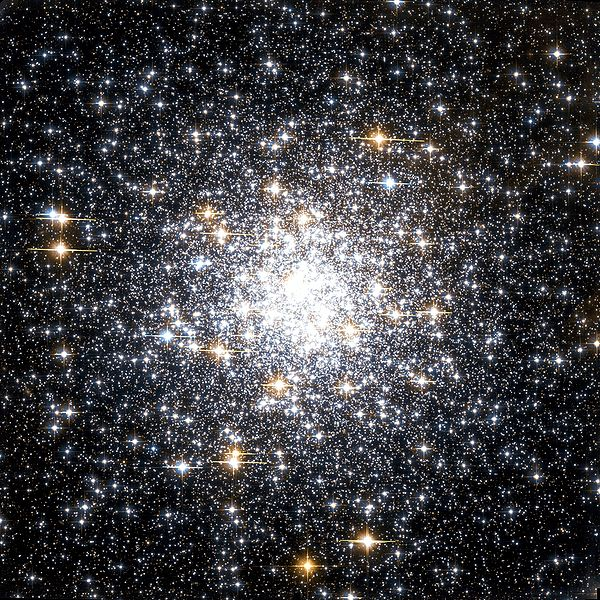
\includegraphics[width=0.8\textwidth]{img/m69}
                \caption{Globular cluster ``Messier 69'' in the constellation Sagittarius.}
                \label{fig:m69}
            \end{figure}
        \end{column}
    \end{columns}
\end{frame}

\begin{frame}
    \frametitle{Introduction}
    \framesubtitle{Motivation (2/2)}

    \begin{columns}
        \begin{column}{0.5\textwidth}
            \begin{itemize}
                \item Evolution of the High Performance Computing (HPC).
            \end{itemize}
            \begin{center}
                
\includegraphics[width=0.8\textwidth]{img/top500}
            \end{center}
        \end{column}
        \begin{column}{0.5\textwidth}
            \begin{figure}
                \centering
                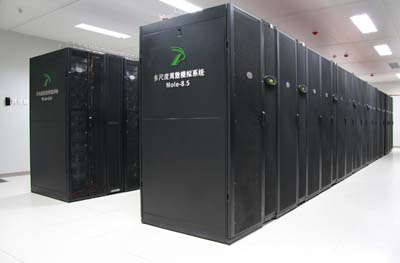
\includegraphics[width=0.8\textwidth]{img/cluster}
                \caption{GPU Cluster Mole-8.5 in Beijing, at the Institute of Process
                         Engineering of Chinese Academy of Sciences.
                         (372 nodes and 2,000 NVIDIA Fermi C2050 GPUs)}
                \label{fig:m69}
            \end{figure}
        \end{column}
    \end{columns}
\end{frame}

\section{The {\nbody} problem}
\begin{frame}
    \frametitle{The {\nbody} problem}
    \framesubtitle{Definition}

    Purely dynamic problem, in which the bodies orbital evolution
    is determined exclusive by the \blue{gravitational interaction},

    \begin{align}
        \bs{\ddot{r}}_{i} &= -G \sum\limits^{N}_{\substack{j=1\\j\neq i}}
                              m_{j} {(\bs{r}_i - \bs{r}_j)\over
                              | \bs{r}_i - \bs{r}_j|^{3}}\label{eq:nbody},
    \end{align}

    \noindent
    where $G$ is the gravitational constant
    ($6.67384\times 10^{-11} m^{3} kg^{-1} s^{-2}$),
    $m_j$ is the mass of the $j$th particle
    and $\bs{r}_j$ the position in \emph{Cartesian} coordinates.
    \begin{block}{\red{Note}}
        We denote vectors by bold fonts.
    \end{block}
\end{frame}


\begin{frame}
    \frametitle{The {\nbody} problem}
    \framesubtitle{Checking the system evolution}

    \begin{itemize}
        \item The \blue{initial condition} are usually the masses,
            position and velocity.

        \item \blue{Chaotic nature}, the evolution of this systems
         will depend of the initial parameters.

        \item The often invariant to check the integration of the system,
            is the system's \blue{energy},

            \begin{align}
                E &= {1 \over 2} \sum\limits^{N}_{i=1} m_{i} \bs{v}_{i}^{2} -
                     \sum\limits_{i=1}^{N} \sum\limits_{j > i}^{N}
                     {G m_{i} m_{j} \over |\bs{r}_{i} - \bs{r}_{j}|},
            \end{align}

            \noindent
            where $\bs{v}_i$ is the velocity of the particle $i$.
    \end{itemize}

\end{frame}


\begin{frame}
    \frametitle{The {\nbody} problem}
    \framesubtitle{Particle's time steps}

    \begin{itemize}
        \item The real scenario, \blue{individual} time steps.
        \begin{itemize}
            \item \red{Hard} scenario for parallel computing.
        \end{itemize}
        \item Forming groups of particles, \blue{block} time steps scheme~\cite{Press86}.
        \begin{itemize}
            \item  This time step scheme is popular among  {\nbody} code,
                like Starlab~\cite{portegies2001, hut2003}, Aarseth {\nbody}
                codes~\cite{Aarseth99, Aarseth03,NitadoriAarseth2012},
                $\phi$GRAPE~\cite{harfst2008},
                which gives us the possibility to check our algorithm behavior.
        \end{itemize}
    \end{itemize}
\end{frame}


\begin{frame}
    \frametitle{Introduction}
    \framesubtitle{{\nbody} algorithms classification}

    \begin{description}
        \item[Collision-less]
            A star just sees the \blue{background potential} of the rest of
            the stellar system.
            A model of this situation is the Barnes-Hut Treecode
            with a complexity $O(N\log N)$~\cite{BarnesHut86}
            or the fast multipole method with $O(N)$~\cite{GreendardThesis}.
            \vspace{0.7cm}
        \item[Collisional (``direct-summation'')]
            One star integrates \blue{all gravitational forces}
            for all stars. This typically scale as $O(N^{2})$.
            A well-known example is the family of algorithm of Aarseth
            the direct-summation {\sc Nbody} integrator~\cite{Aarseth99,Spurzem1999,Aarseth03}
            or {\sc kira} code~\cite{PortegiesZwartEtAl01}.
    \end{description}

\end{frame}

\section{Computational aspects}
\begin{frame}
    \frametitle{Introduction}
    \framesubtitle{The computational challenge}

    \begin{itemize}
        \item The {\nbody} codes evolution is related to the available
                \blue{hardware} in our time.
        \item The algorithms with a complexity of $O(N^{2})$ or $O(N^{3})$ require
                \red{supercomputers}.
        \begin{itemize}
            \item  e.g \blue{beowulf clusters},
                which require a parallelization of the code
                ({\sc Nbody6++} developed by Spurzem et al.~\cite{Spurzem1999}).

            \item Special-purpose hardware, like the \blue{GRAPE} (short for GRAvity
                PipE system~\cite{TMFES96,MT98,Makino98,GRAPE6A}.

        \end{itemize}

        \item  The literature overview reveals a strong interest on porting the existing codes to the
            \blue{GPU} architecture, like e.g. the work
            of~\cite{Portegies2007a,Hamada2007,Belleman2008}
            on single nodes or using large
            clusters~\cite{berczik2011high,NitadoriAarseth2012,Capuzzo-DolcettaEtAl2013}.

    \end{itemize}

\end{frame}

\subsection{GPU Computing}
\begin{frame}
    \frametitle{Introduction}
    \framesubtitle{GPU Computing}

    \begin{columns}
        \begin{column}{0.6\textwidth}
            \begin{itemize}
                \item \emph{``Using a GPU (Graphic Processing Unit) together with
                      a CPU to accelerate scientific calculation operations
                      or general purpose calculation''}
            \end{itemize}
        \end{column}
        \begin{column}{0.4\textwidth}
             \begin{figure}
                 \centering
                 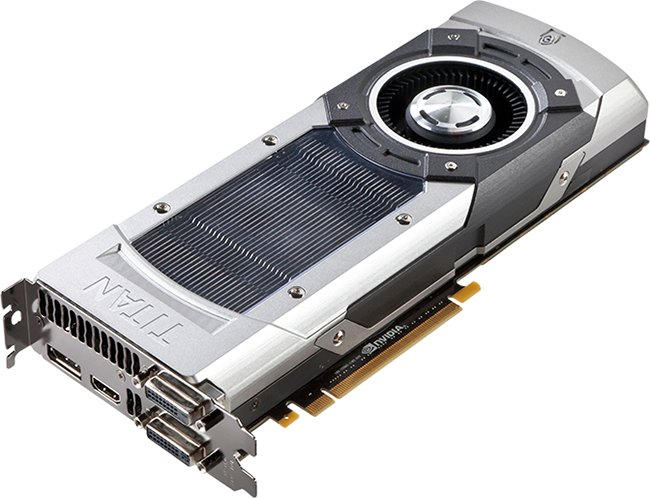
\includegraphics[width=0.8\textwidth]{img/titan}
                 \caption{NVIDIA\textsuperscript{\textregistered} GTX Titan}
                 \label{fig:titan}
             \end{figure}
        \end{column}
    \end{columns}
\end{frame}

\begin{frame}
    \frametitle{Introduction}
    \framesubtitle{CPU/GPU Design}

    \begin{itemize}
        \item CPU,
        \begin{itemize}
            \item Designed to have a good \blue{performance}
                  in parallel and non-parallel scenarios.
            \item Minimizes the \blue{latency} experimented by a thread
                  (large cache memory)
        \end{itemize}
        \item GPU,
            \begin{itemize}
            \item Designed to perform highly parallel work.
            \item Maximizes the \blue{throughput} of all the threads.
            \end{itemize}
    \end{itemize}

    \begin{footnotesize}
        \begin{columns}
            \begin{column}{0.35\textwidth}
            \begin{block}{Performance}
                Capacity of perform individual instructions in a certain time.
            \end{block}
            \end{column}
            \begin{column}{0.3\textwidth}
            \begin{block}{Latency}
                Measure of time delay experienced in a system.
            \end{block}
            \end{column}
            \begin{column}{0.3\textwidth}
            \begin{block}{Throughput}
                Capacity of perform a whole task in a certain time.
            \end{block}
            \end{column}
        \end{columns}
    \end{footnotesize}

    %\begin{description}
    %    \item[Performance]
    %            Capacity of perform individual instructions in a certain time.
    %    \item[Throughput]
    %            Capacity of perform a whole task in a certain time.
    %    \item[Latency]
    %            Measure of time delay experienced in a system.
    %    \item[Granularity]
    %            Break down a system into small parts.(Coarse and Fine)
    %\end{description}
\end{frame}

\begin{frame}
    \framesubtitle{Introduction}
    \frametitle{GPU Architecture}

    \begin{columns}
        \begin{column}{0.5\textwidth}
            \begin{block}{Task parallelism}
                Each processor perform a different task.
            \end{block}
            \begin{block}{Data parallelism}
                Each processor perform the same task, but not on the same data set.
            \end{block}
        \end{column}
        \begin{column}{0.5\textwidth}
             \begin{figure}
                 \centering
                 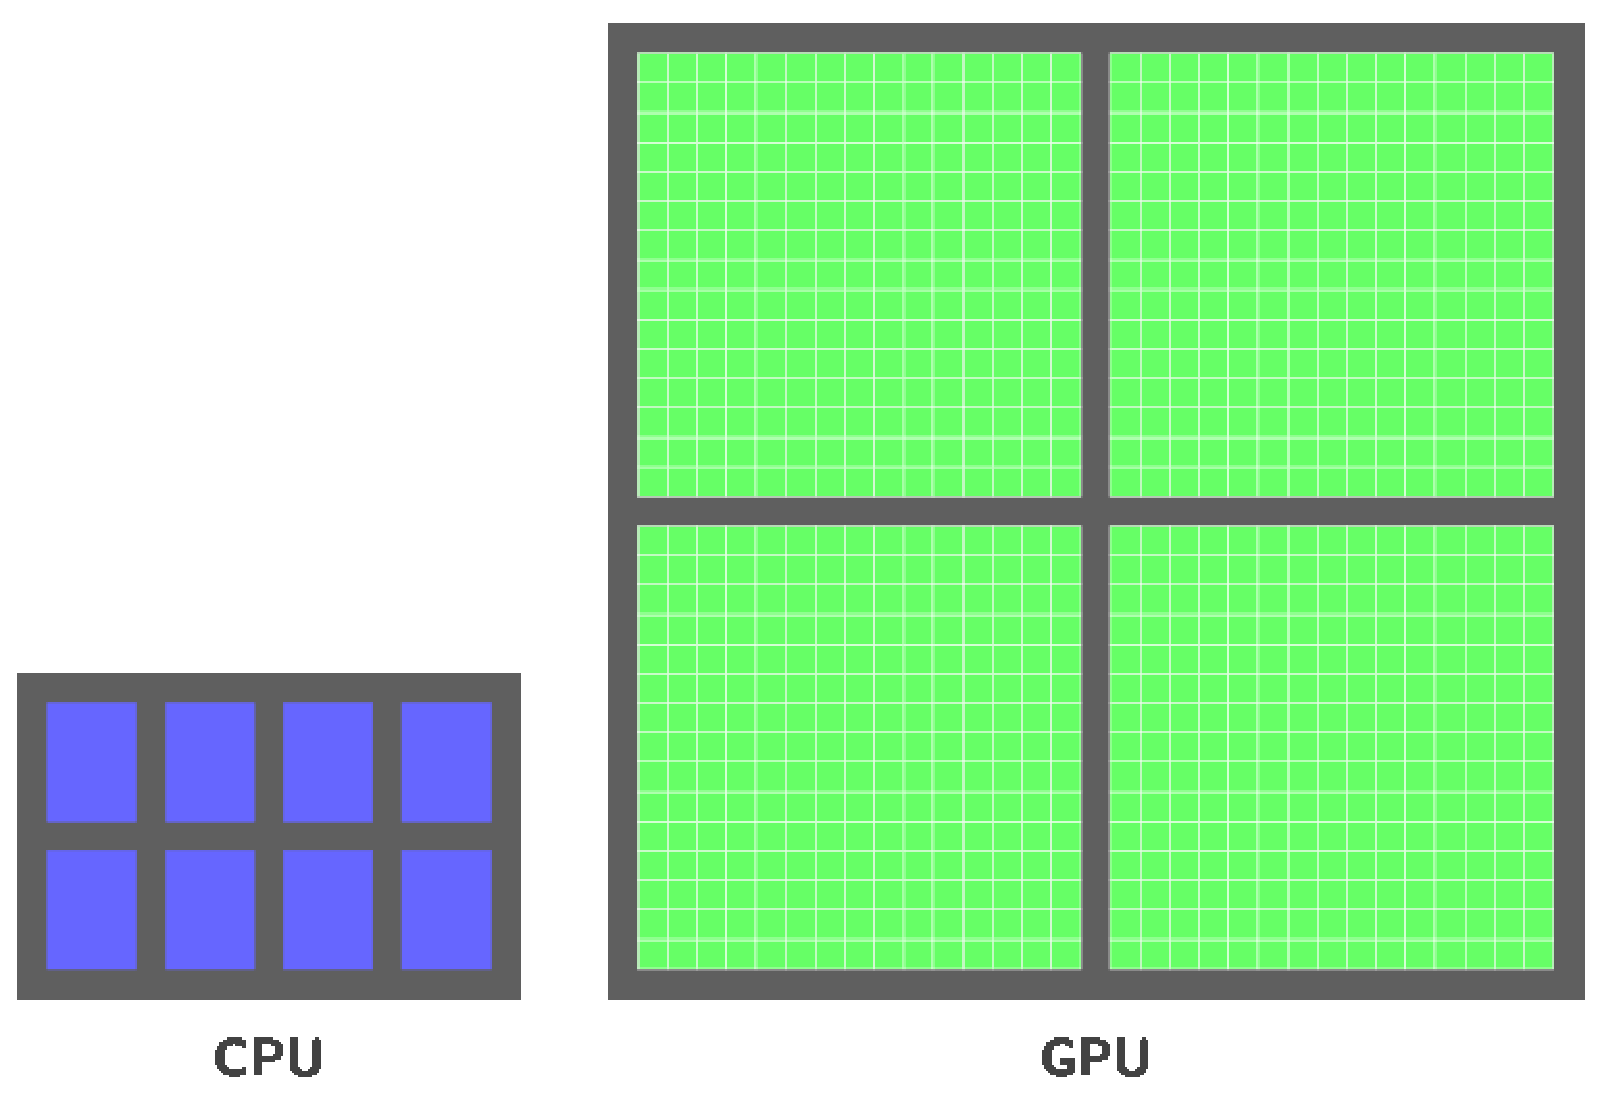
\includegraphics[width=0.8\textwidth]{img/cpu_gpu}
                 \caption{GPU and CPU core scheme}
                 \label{fig:titan}
             \end{figure}
        \end{column}
    \end{columns}
\end{frame}

\subsection{Programming strategy}
\begin{frame}
    \frametitle{Introduction}
    \framesubtitle{Programming strategy}

    \begin{columns}
        \begin{column}{0.5\textwidth}
            \begin{figure}
                \captionsetup{singlelinecheck=off}
                \centering
                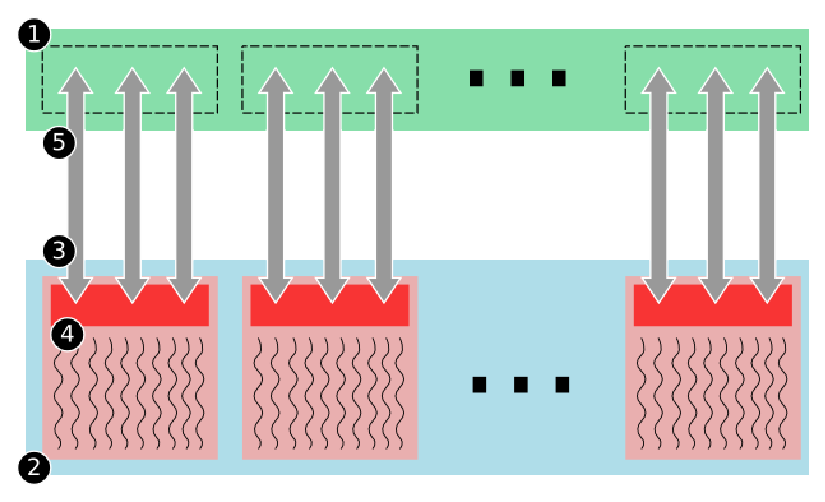
\includegraphics[width=0.9\textwidth]{img/cuda-strategy}
                \label{fig:estrategia}
                \caption{CUDA Programming strategy}
            \end{figure}
        \end{column}
        \begin{column}{0.5\textwidth}
             \begin{enumerate}
                 \item CPU memory allocation,
                 \item \dgreen{GPU} memory allocation,
                 \item Data copying,  CPU $\rightarrow$ \dgreen{GPU},
                 \item Task execution on the data,
                 \item Data copying, \dgreen{GPU} $\rightarrow$ CPU,
             \end{enumerate}
        \end{column}
    \end{columns}
\end{frame}


\section{The $N-$body problem}
\begin{frame}
    \frametitle{The {\nbody} problem}
    \framesubtitle{Definition}

    Purely dynamic problem, in which the bodies orbital evolution
    is determined exclusive by the \blue{gravitational interaction},

    \begin{align}
        \bs{\ddot{r}}_{i} &= -G \sum\limits^{N}_{\substack{j=1\\j\neq i}}
                              m_{j} {(\bs{r}_i - \bs{r}_j)\over
                              | \bs{r}_i - \bs{r}_j|^{3}}\label{eq:nbody},
    \end{align}

    \noindent
    where $G$ is the gravitational constant
    ($6.67384\times 10^{-11} m^{3} kg^{-1} s^{-2}$),
    $m_j$ is the mass of the $j$th particle
    and $\bs{r}_j$ the position in \emph{Cartesian} coordinates.
    \begin{block}{\red{Note}}
        We denote vectors by bold fonts.
    \end{block}

\end{frame}


\begin{frame}
    \frametitle{The {\nbody} problem}
    \framesubtitle{Checking the system evolution}

    \begin{itemize}
        \item The \blue{initial condition} are usually the masses,
            position and velocity.

        \item \blue{Chaotic nature}, the evolution of this systems
         will depend of the initial parameters.

        \item The often invariant to check the integration of the system,
            is the system's \blue{energy},

            \begin{align}
                E &= {1 \over 2} \sum\limits^{N}_{i=1} m_{i} \bs{v}_{i}^{2} -
                     \sum\limits_{i=1}^{N} \sum\limits_{j > i}^{N}
                     {G m_{i} m_{j} \over |\bs{r}_{i} - \bs{r}_{j}|},
            \end{align}

            \noindent
            where $\bs{v}_i$ is the velocity of the particle $i$.
    \end{itemize}

\end{frame}


\begin{frame}
    \frametitle{The {\nbody} problem}
    \framesubtitle{Particle's time steps}

    \begin{itemize}
        \item The real scenario, \blue{individual} time steps.
        \begin{itemize}
            \item \red{Hard} scenario for parallel computing.
        \end{itemize}
        \item Forming groups of particles, \blue{block} time steps scheme~\cite{Press86}.
        \begin{itemize}
            \item  This time step scheme is popular among  {\nbody} code,
                like Starlab~\cite{portegies2001, hut2003}, Aarseth {\nbody}
                codes~\cite{Aarseth99, Aarseth03,NitadoriAarseth2012},
                $\phi$GRAPE~\cite{harfst2008},
                which gives us the possibility to check our algorithm behavior.
        \end{itemize}
    \end{itemize}
\end{frame}


\section{GPU Computing}
\begin{frame}
    \frametitle{GPU Computing}
    \framesubtitle{Introduction}

    \begin{columns}
        \begin{column}{0.5\textwidth}
            \begin{itemize}
                \item \emph{``Using a GPU (Graphic Processing Unit) together with
                      a CPU to accelerate scientific calculation operations
                      or general purpose calculation''}
            \end{itemize}
        \end{column}
        \begin{column}{0.5\textwidth}
             \begin{figure}
                 \centering
                 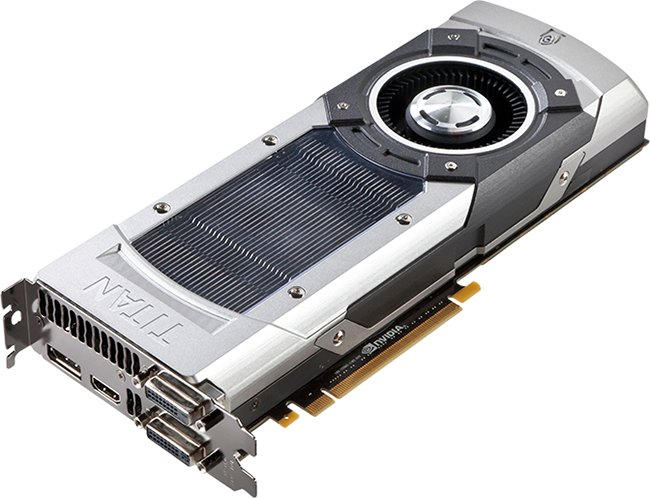
\includegraphics[width=0.8\textwidth]{img/titan}
                 \caption{NVIDIA\textsuperscript{\textregistered} GTX Titan}
                 \label{fig:titan}
             \end{figure}
        \end{column}
    \end{columns}
\end{frame}

\begin{frame}
    \frametitle{GPU Computing}
    \framesubtitle{Features}

    \begin{itemize}
        \item CPU,
        \begin{itemize}
            \item Designed to have a good \blue{performance}
                  in parallel and non-parallel scenarios.
            \item Minimizes the \blue{latency} experimented by a thread
                  (large cache memory)
        \end{itemize}
        \item GPU,
            \begin{itemize}
            \item Designed to perform highly parallel work.
            \item Maximizes the \blue{throughput} of all the threads.
            \end{itemize}
    \end{itemize}

    \begin{footnotesize}
        \begin{columns}
            \begin{column}{0.35\textwidth}
            \begin{block}{Performance}
                Capacity of perform individual instructions in a certain time.
            \end{block}
            \end{column}
            \begin{column}{0.3\textwidth}
            \begin{block}{Latency}
                Measure of time delay experienced in a system.
            \end{block}
            \end{column}
            \begin{column}{0.3\textwidth}
            \begin{block}{Throughput}
                Capacity of perform a whole task in a certain time.
            \end{block}
            \end{column}
        \end{columns}
    \end{footnotesize}

    %\begin{description}
    %    \item[Performance]
    %            Capacity of perform individual instructions in a certain time.
    %    \item[Throughput]
    %            Capacity of perform a whole task in a certain time.
    %    \item[Latency]
    %            Measure of time delay experienced in a system.
    %    \item[Granularity]
    %            Break down a system into small parts.(Coarse and Fine)
    %\end{description}
\end{frame}

\begin{frame}
    \frametitle{GPU Computing}
    \framesubtitle{Architecture}

    \begin{columns}
        \begin{column}{0.5\textwidth}
            \begin{block}{Task parallelism}
                Each processor perform a different task.
            \end{block}
            \begin{block}{Data parallelism}
                Each processor perform the same task, but not on the same data set.
            \end{block}
        \end{column}
        \begin{column}{0.5\textwidth}
             \begin{figure}
                 \centering
                 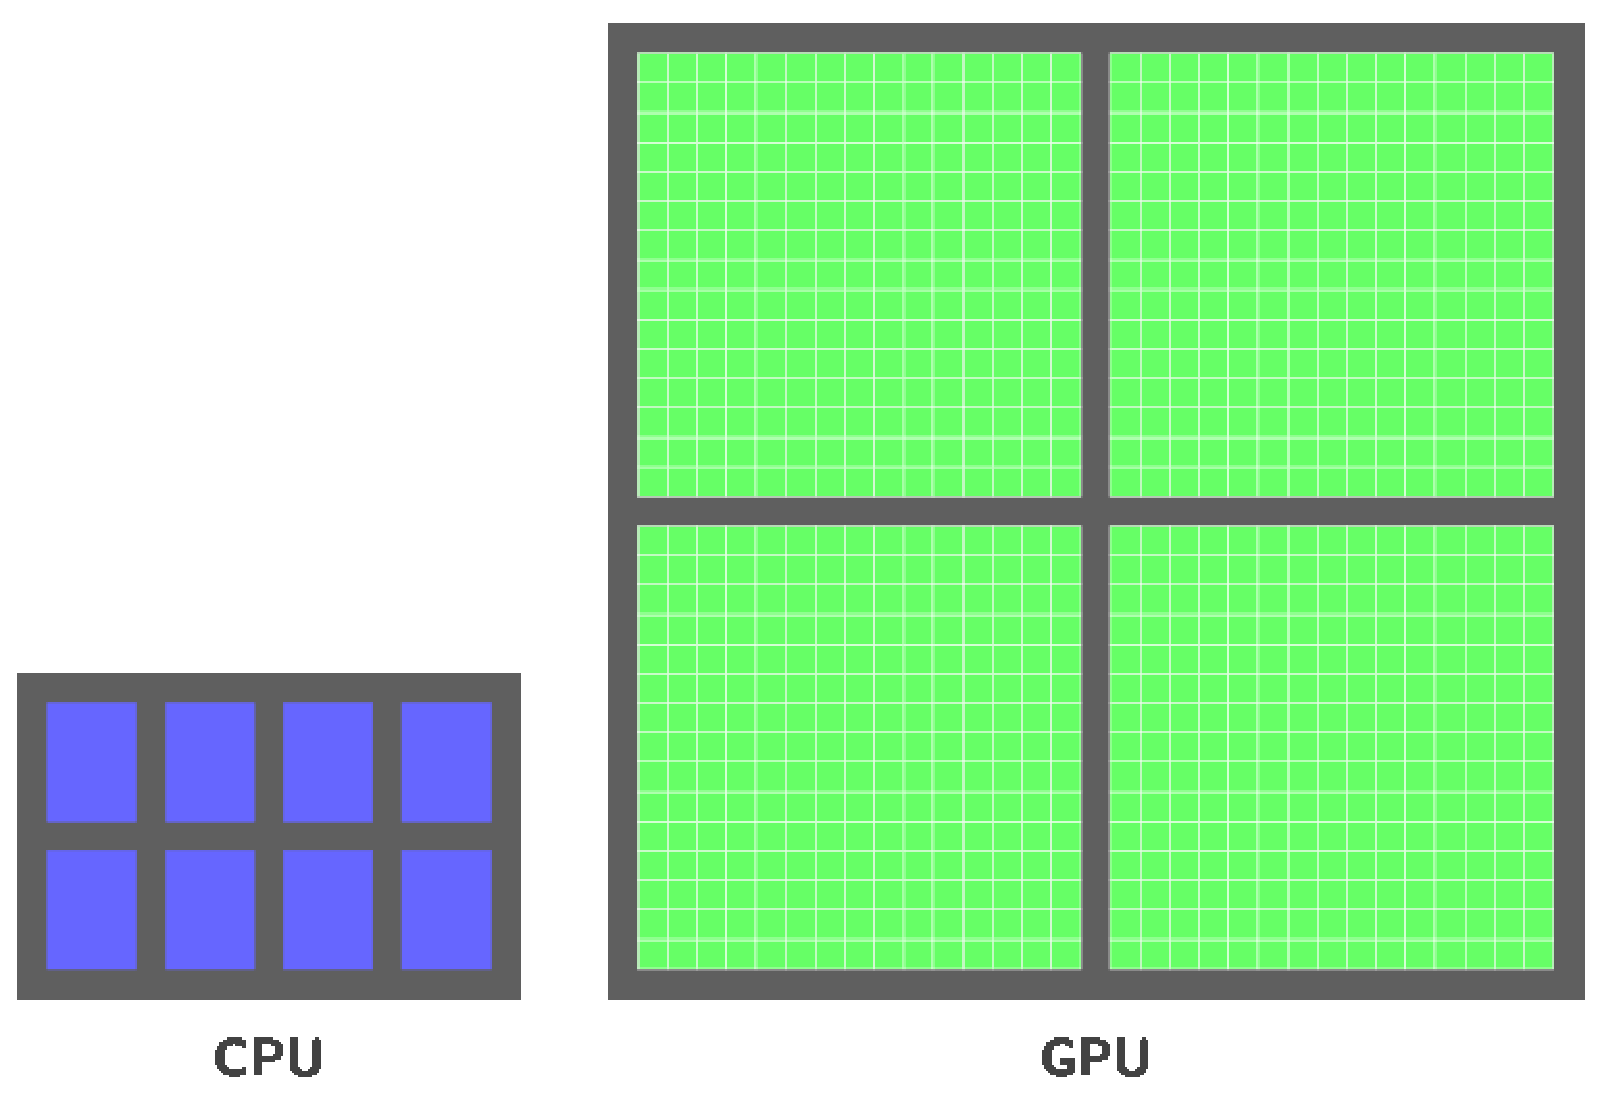
\includegraphics[width=0.8\textwidth]{img/cpu_gpu}
                 \caption{GPU and CPU core scheme}
                 \label{fig:titan}
             \end{figure}
        \end{column}
    \end{columns}
\end{frame}

\begin{frame}
    \frametitle{GPU Computing}
    \framesubtitle{Functionality}

    \begin{columns}
        \begin{column}{0.5\textwidth}
            \begin{figure}
                \captionsetup{singlelinecheck=off}
                \centering
                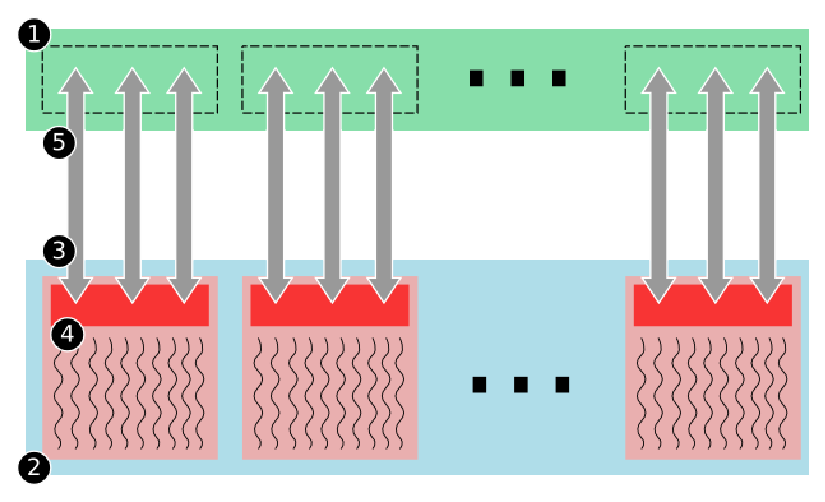
\includegraphics[width=0.9\textwidth]{img/cuda-strategy}
                \label{fig:estrategia}
                \caption{CUDA Programming strategy}
            \end{figure}
        \end{column}
        \begin{column}{0.5\textwidth}
             \begin{enumerate}
                 \item CPU memory allocation,
                 \item \dgreen{GPU} memory allocation,
                 \item Data copying,  CPU $\rightarrow$ \dgreen{GPU},
                 \item Task execution on the data,
                 \item Data copying, \dgreen{GPU} $\rightarrow$ CPU,
             \end{enumerate}
        \end{column}
    \end{columns}
\end{frame}



\section{Implementation}
\begin{frame}
    \frametitle{Parallelization scheme}
    \framesubtitle{$j-$parallelization scheme}

    Our configuration is based in the idea presented in~\cite{NitadoriAarseth2012},

    \begin{center}
    \begin{figure}[H]
        \centering
    \colorbox{white}{
        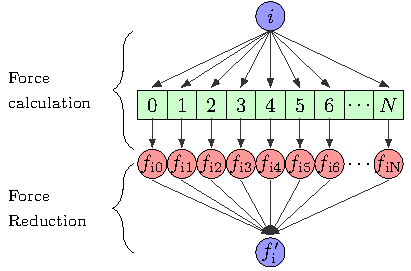
\includegraphics[width=0.55\textwidth]{img/force_split_reduction.pdf}
    }
        \caption{Parallelization scheme to split the $j-$loop instead of the $i-$loop.
                 In this case, we have two sections, the first is to calculate
                 the force interactions of the $i-$particle with the whole
                 system but by different threads. Then a reduction (sum) is necessary
                 to get the new value for the $i-$particle force.}
        \label{fig:force_split_reduction}
    \end{figure}
    \end{center}

\end{frame}

\begin{frame}
    \frametitle{Implementation}
    \framesubtitle{Class diagram}
    \begin{center}
        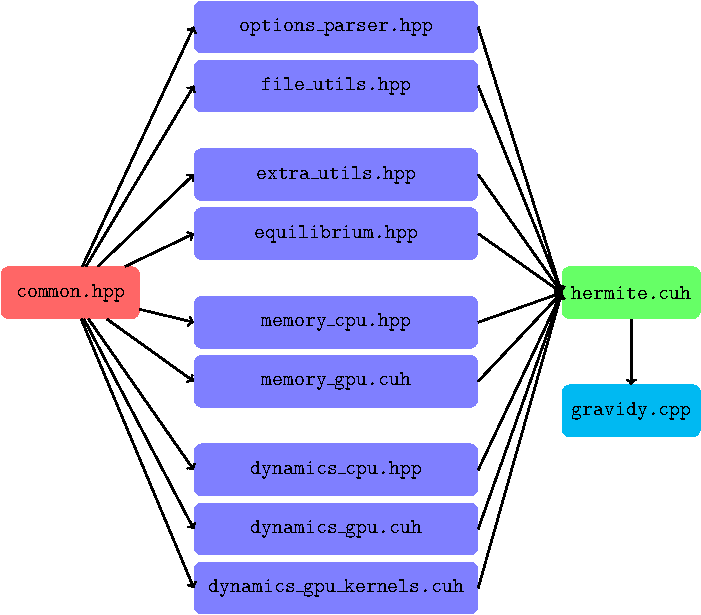
\includegraphics[height=0.8\textheight]{img/files_structure.pdf}
    \end{center}
\end{frame}



\section{Experiments}
\begin{frame}
    \frametitle{Experiments}
    \framesubtitle{Integrator scaling}

\begin{figure}[H]
    \centering
    \label{fig:time}
    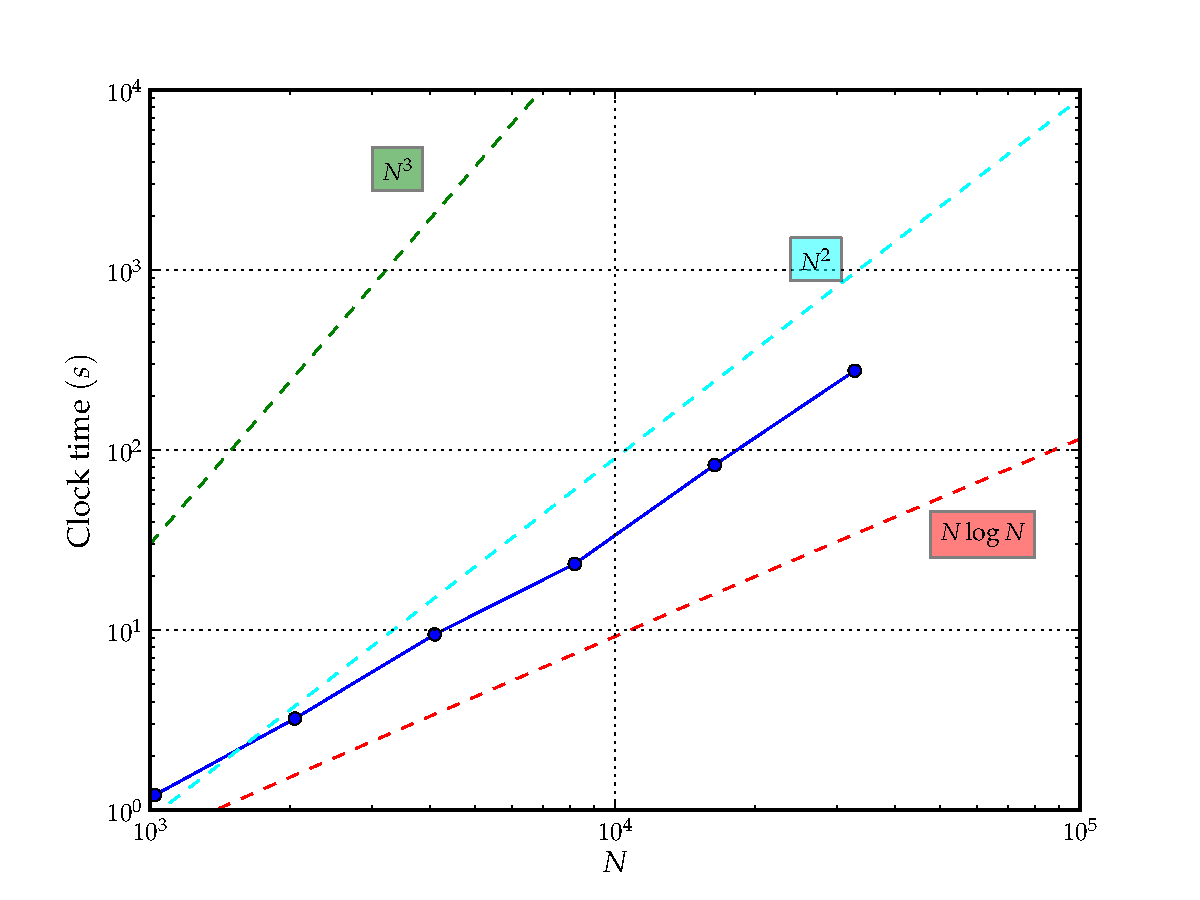
\includegraphics[width=0.65\textwidth]{img/test_time-1t-N.pdf}
    \caption{Clock time of integration up to $t=1$ NBU using $\eta = 0.01$ and
             $\epsilon = 10^{-4}$ using different amount of particles.}
\end{figure}

\end{frame}
\begin{frame}
    \frametitle{Experiments}
    \framesubtitle{Clock time comparison}

\begin{table}[H]
    \centering
    \footnotesize
    \begin{tabular}{rrrrr}
        \hline
        {\bf N} & \multicolumn{1}{c}{\bf CPU}
                & \multicolumn{1}{c}{\bf CPU + OpenMP}
                & \multicolumn{1}{c}{\bf CPU + GPU}
                & \multicolumn{1}{c}{\bf GPU}   \\
                & (single thread) & (many threads)     & (mixed approach) &  (multi threads) \\ \hline
         {\bf  1k} &    12.98 [s] &   8.19 [s] &    3.57 [s]           &    1.21 [s]          \\
         {\bf  2k} &    61.32 [s] &  34.94 [s] &   13.42 [s]           &    3.22 [s]          \\
         {\bf  4k} &   282.98 [s] & 162.64 [s] &   54.28 [s]           &    9.45 [s]          \\
         {\bf  8k} &  1227.40 [s] & 682.56 [s] &  208.91 [s]           &   23.31 [s]          \\
         {\bf 16k} &  5542.35 [s] & 3227.91 [s] &  904.82 [s]           &   82.63 [s]          \\
         {\bf 32k} & 26383.71 [s] & 15076.40 [s] & 3722.92 [s]           &  275.53 [s]          \\ \hline
    \end{tabular}
    \caption{Clock time foreach integrator version.}
    \label{tab:acc}
\end{table}

\end{frame}

\begin{frame}
    \frametitle{Experiments}
    \framesubtitle{Clock time comparison}

\begin{figure}[H]
    \centering
    \label{fig:acc}
    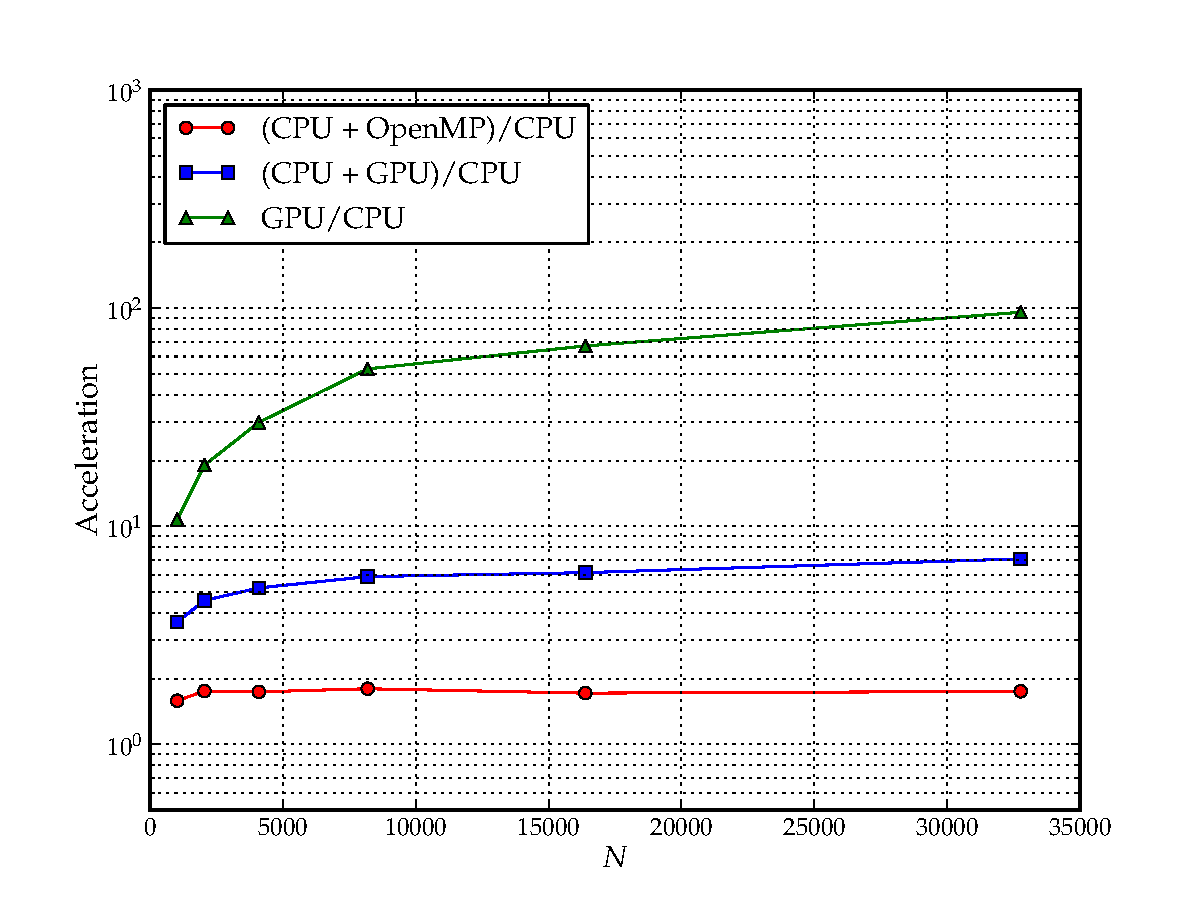
\includegraphics[width=0.7\textwidth]{img/test_gpu-acceleration.pdf}
    \caption{Acceleration between the implementations described in Table~\ref{tab:acc}}
\end{figure}

\end{frame}
\begin{frame}
    \frametitle{Experiments}
    \framesubtitle{Integrator Performance}
\begin{figure}[H]
    \centering
    \label{fig:gflops}
    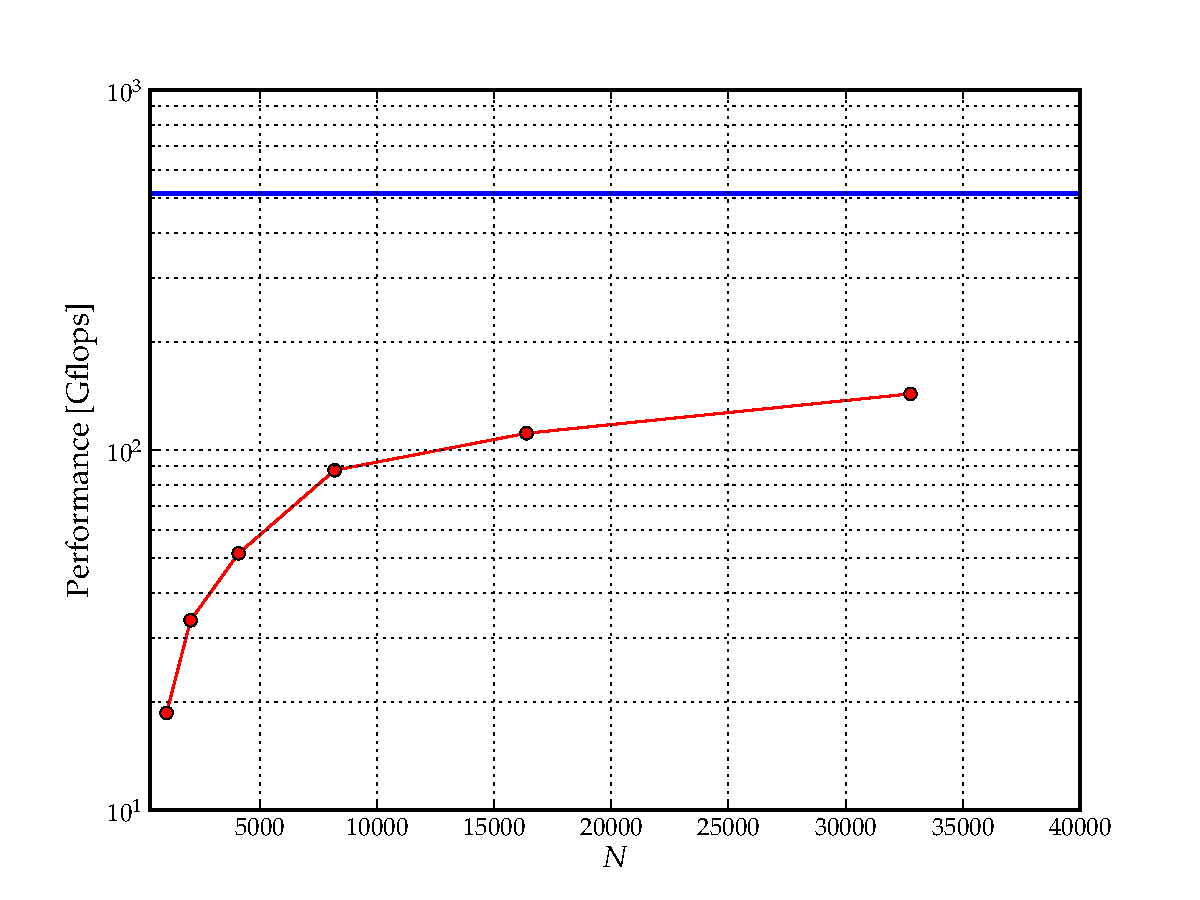
\includegraphics[width=0.65\textwidth]{img/test_gflops.pdf}
    \caption{GPU gravitational interactions performance in GFLOPS for different amount of particles.}
\end{figure}

\end{frame}


\section{Challenges and future work}
\begin{frame}
    \frametitle{Challenges and future work}

    We presented a first version of our new {\nbody} code,
    written purely in C/C++ and CUDA, called \red{\GR}.

    \begin{itemize}
        \item The current version of our code,
        \begin{itemize}
            \item evolves a globular cluster, using and \blue{Hermite 4th order}
                integration scheme, using block time steps.
            \item has a \blue{suitable} in the energy conservation,
                reaching errors around $\approx 10^{-9}$ and $\approx 10^{-7}$-
        \end{itemize}
    \end{itemize}

\end{frame}

\begin{frame}
    \frametitle{Challenges and future work}
    \framesubtitle{Features}

    \begin{itemize}
        \item Iterative and incremental development (APOD cycle),
        \item Modular code,
        \item Documentation,
        \item Hermite 4th order integrator scheme,
        \item Block time steps,
        \item GPU computing to improve the hot-spots,
    \end{itemize}
\end{frame}

\begin{frame}
    \frametitle{challenges and future work}
    \framesubtitle{the next steps (1/2)}

    \begin{itemize}
%        \item Publication in the ISI Journal ``Monthly Notices of the Royal Astronomical Society (MNRAS)''.
        \item Continue the \blue{research} on {\nbody} integrators, like
                higher order Hermite schemes.
        \item More physical phenomena treatments,
        \begin{itemize}
            \item \blue{Neighbors treatment}, to handle the binary formation,
                This has been proved by using a time-symmetric integration scheme
                for the binary system, which is described in the work of~\cite{myriad}.

            \item Handle \blue{semi-Keplerian} systems,
                    {\nbody} systems with a central massive particle~\cite{ulf},
                    like a massive black hole (MBH) in the galactic center,
                    or a star in a protoplanetary system, etc.

            \item Post-Newtonian terms into the acceleration and its derivatives.
        \end{itemize}
    \end{itemize}
\end{frame}

\begin{frame}
    \frametitle{challenges and future work}
    \framesubtitle{the next steps (2/2)}

    \begin{itemize}
        \item Porting the code towards large GPU clusters, \blue{multi-GPU} environment.
        \item Studying \blue{new computational improvements},
        \begin{itemize}
            \item Numerical precision,
            \item Mixed-parallel schemes,
            \item Different architectures,
        \end{itemize}
        \item Use GPU Computing to solve additional Astrophysical problems,
        \begin{itemize}
            \item Smoothed-particle hydrodynamics (SPH).
        \end{itemize}

    \end{itemize}
\end{frame}



%\section{Acknowledgements}
%
\begin{frame}
    \frametitle{Acknowledgements}

    \begin{itemize}
%        \item Dr. Luis Salinas, Dr. Héctor Allende and Dr. Jorge Cuadra (Committee).
%        \item Dr. Pau Amaro-Seoane (AEI).
        \item {\bf $N-$body community},
                Sverre Aarseth,
                Holger Baumgardt,
                Peter Berczik,
                Douglas Heggie,
                Piet Hut,
                Patrick Brem,
                Simos Konstantinidis,
                Keigo Nitadori,
                Ulf L{\"o}ckmann,
                Rainer Spurzem, etc.
%        \item Master scholaships program,
%              \emph{``Comisión Nacional de Investigación Científica y Tecnológica de Chile'' (CONICYT)}
%        \item Transregio 7 ``Gravitational Wave Astronomy'',
%              \emph{Deutsche Forschungsgemeinschaft (DFG)}

    \end{itemize}

\end{frame}


% References
\begin{frame}[allowframebreaks]
\footnotesize

\bibliographystyle{ieeetr}            %
\bibliography{/home/cmaureir/repos/GraviDy-docs/bib/tesis,/home/cmaureir/repos/GraviDy-docs/bib/aamnem99,/home/cmaureir/repos/GraviDy-docs/bib/biblio,/home/cmaureir/repos/GraviDy-docs/bib/cuda}    %
\end{frame}

% Final slide
\begin{frame}[t,plain]
\titlepage
\end{frame}

\end{document}
